\documentclass[
	11pt,
]{beamer}

\newcommand\myheading[1]{%
  \par\bigskip
  {\Large\bfseries#1}\par\smallskip}


\graphicspath{{Images/}{./}} 

\usepackage{booktabs} 

%----------------------------------------------------------------------------------------
%	SELECT LAYOUT THEME
%----------------------------------------------------------------------------------------

\usetheme{CambridgeUS}

%----------------------------------------------------------------------------------------
%	SELECT COLOR THEME
%----------------------------------------------------------------------------------------

\usecolortheme{seahorse}

%----------------------------------------------------------------------------------------
%	SELECT FONT THEME & FONTS
%----------------------------------------------------------------------------------------

\usefonttheme{default} % Typeset using the default sans serif font

%------------------------------------------------

\usepackage{palatino} % Use the Palatino font for serif text

\usepackage[default]{opensans} % Use the Open Sans font for sans serif text

%----------------------------------------------------------------------------------------
%	SELECT INNER THEME
%----------------------------------------------------------------------------------------

\useinnertheme{circles}

%----------------------------------------------------------------------------------------
%	PRESENTATION INFORMATION
%----------------------------------------------------------------------------------------

\title[Parareal Algorithm]{\\ \textbf{Parareal Algorithm}}


\author[O. BOUHENNICHE \and N. ZAOUACHE]{Oussama BOUHENNICHE \and Narimane ZAOUACHE}

\institute[]{University of Strasbourg}


\date[\today]{ CSMI \\ \today}

%----------------------------------------------------------------------------------------

\begin{document}

%----------------------------------------------------------------------------------------
%	TITLE SLIDE
%----------------------------------------------------------------------------------------

\begin{frame}
	\titlepage
\end{frame}

%----------------------------------------------------------------------------------------
%	TABLE OF CONTENTS SLIDE
%----------------------------------------------------------------------------------------

\begin{frame}
	\frametitle{Presentation Overview}

	\tableofcontents
\end{frame}
%----------------------------------------------------------------------------------------
%	PRESENTATION BODY SLIDES
%----------------------------------------------------------------------------------------


\section{Parareal algorithm}

%------------------------------------------------
\begin{frame}
	\frametitle{Parareal algorithm}
	Parareal is a parallel algorithm from numerical analysis and used for
	the solution of initial value problems\cite{lions2001resolution}.

	\begin{columns}[c]
		\begin{column}{\textwidth}
			\begin{itemize}
				\item Was introduced in 2001 by Lions, Maday and Turinici.
				\item Has become one of the most widely studied parallel-in-time integration methods.
			\end{itemize}
		\end{column}
	\end{columns}

\end{frame}

%------------------------------------------------

\section{Context and objectives}

%------------------------------------------------
\begin{frame}
	\frametitle{Context and Objectives}
	\myheading{Context}


	the development of the parareal algorithm in feel++ in parallel and in C++.

	\myheading{Objectives}

	\begin{columns}[c]
		\begin{column}{\textwidth}
			\begin{itemize}
				\item Study parareal algorithm.
				\item Study a parallel version of parareal algorithm.
				\item Use Lorenz System\cite{lorenz1963deterministic} as test case.
				\item Compare different ode solvers and parareal.
				\item Implement parallel version of parareal algorithm.
				\item Study the possibility of use parareal with feel++.
				\item Implement use of parareal with feel++ (if applicable).
			\end{itemize}
		\end{column}

	\end{columns}

\end{frame}

%------------------------------------------------

\section{Roadmap}
\begin{frame}
	\frametitle{Roadmap}
	\begin{columns}[c]
		\begin{column}{\textwidth}
			\begin{itemize}
				\item Implement Lorenz Model for order 1 and 4 using constant time steppin and add support for Lorenz results visualisation.
				\item Study sundials and scipy.ode with constant and adaptive time stepping.
				\item Study parareal algorithm and Implement initial version of parareal in sequential.
				\item Compare different ode solvers and parareal on Lorenz system.
				\item Study and Implement a parallel version of parareal algorithm.
				\item Study the possibility of use parareal with feel++.
				\item Implement use of parareal with feel++ (if applicable).
			\end{itemize}
		\end{column}
	\end{columns}
\end{frame}

\begin{frame}
	\frametitle{Github Roadmap}
	\begin{figure}
		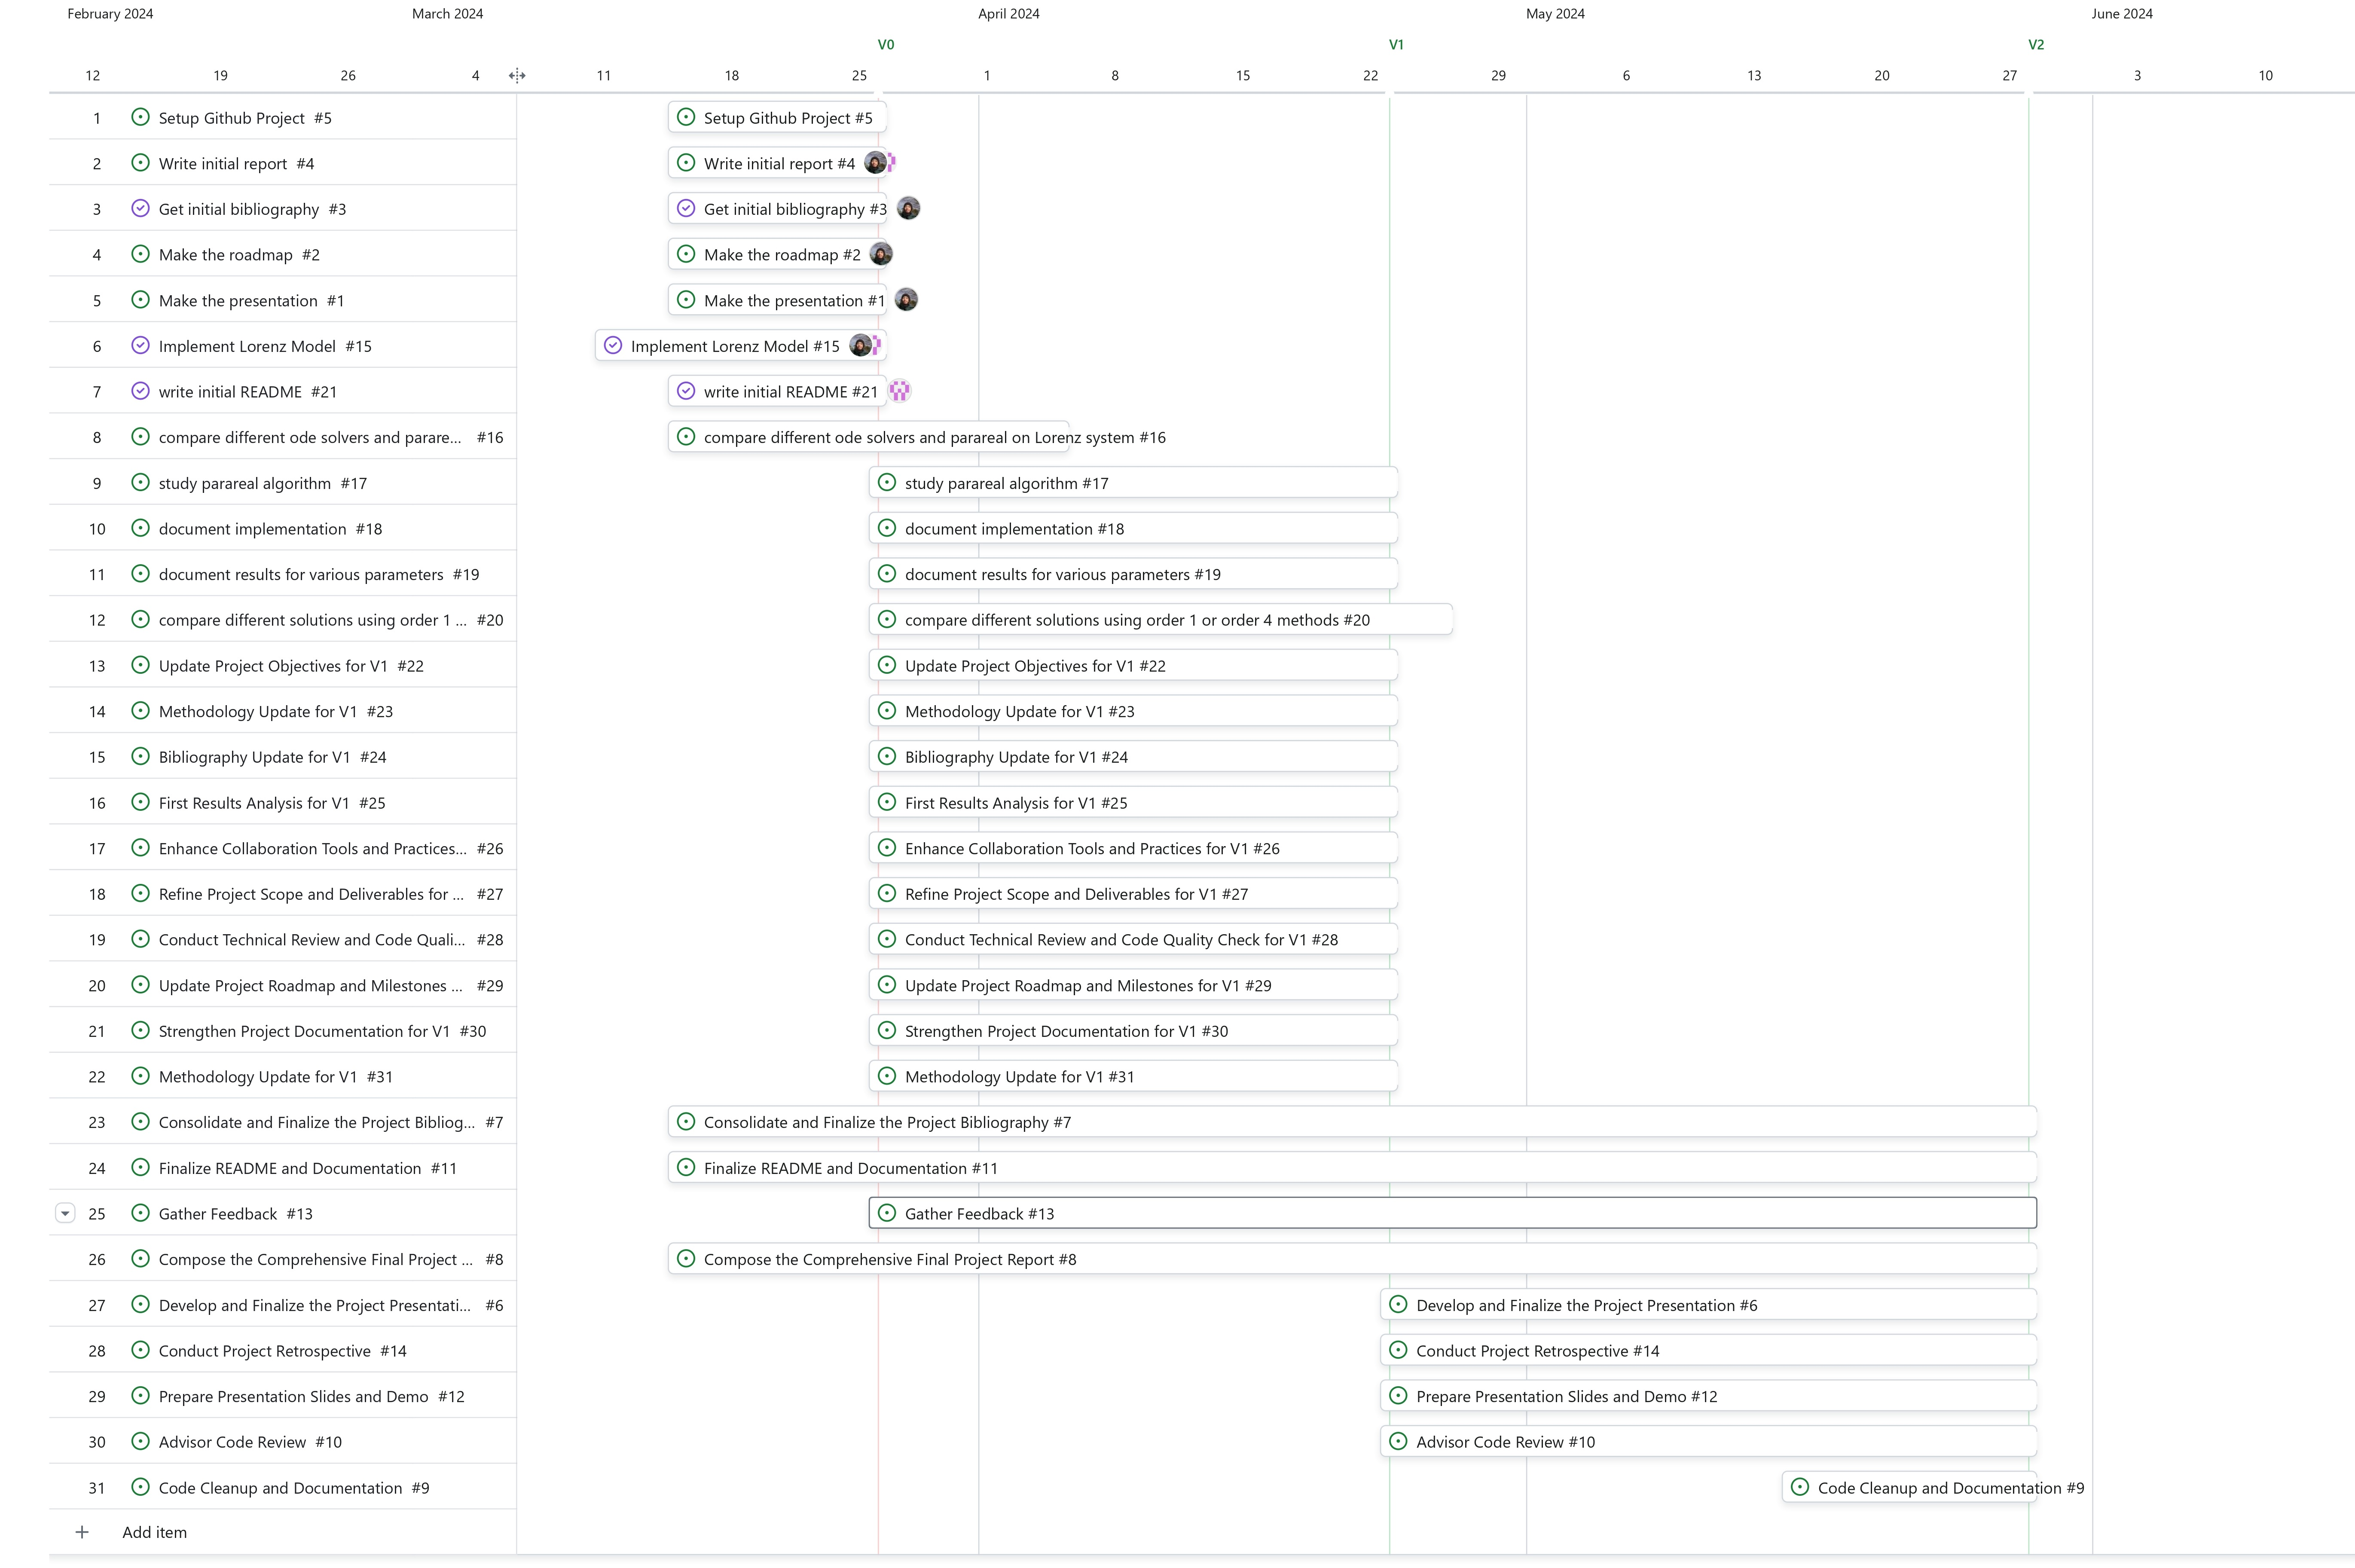
\includegraphics[width=.90\linewidth]{roadmap.jpg}
	\end{figure}
\end{frame}

%------------------------------------------------

\section{References}

\begin{frame}[allowframebreaks]
	\frametitle{References}
	\bibliographystyle{plain}
	\bibliography{../References}
  \end{frame}

%------------------------------------------------

\begin{frame}
	\begin{center}
		{\Huge The End}

		\bigskip\bigskip

		{\LARGE Questions? Comments?}
	\end{center}
\end{frame}

%----------------------------------------------------------------------------------------


\end{document}